\section{Comparison}
In order to compare two works, we decided to use the clustering \gls{fcm}, which is less dependent on possible noise, especially since the comparison between two works will leverage smaller densities and therefore noise could pollute the results.

\noindent In this subsection, we will look in detail at the algorithm for comparing works and see an example application to better investigate its characteristics.

\paragraph{Definitions}
As already mentioned in \cref{chap:LiteratureReview}, the comparison between two distributions $\mathcal{A}$, $\mathcal{B}$ will pass through the use of a clustering algorithm.

\noindent In particular, we used the \gls{kmeans} to implement a clusterisation that discretized the space. Finally, over this discretisation we applied this definition of distance:
\begin{equation}
	\label{eq:kmeans_dist}
	d(\mathcal{A},\mathcal{B})=(1+J_{D_\mathcal{A},D_\mathcal{B}})^{-1}\frac{1}{\mu(D_\mathcal{A}\cup D_\mathcal{B})}\int d\mu(c) \left(\frac{r(c)-1}{r(c)+1}\right)^2
\end{equation}

\noindent Now, we will apply \gls{fcm} to the fused distribution $\mathcal{L}$. For each cluster with centroid $c$, we will compute the size $\mu(c)$ and the density of the set of samples $d_{A}(c)$, $d_{B}(c)$. Finally, we will give a definition of a Jaccard index between dictionaries $D_A$ and $D_B$ using the fuzzy logic.

\noindent Since \gls{fcm} is a generalisation of \gls{kmeans}, let us try to define these quantities starting from \gls{kmeans}. In particular, we define the weight of a cluster as a quantity proportional to the $k$-dimensional hypervolume of a hypersphere having radius the mean square distance of the data from its centroid:
\begin{equation*}
	\mu(c) = {\sqrt{\mathbb{E}_{x\sim\mathcal{L}}\left[\left\|x-c\right\|^2\middle|\mathcal{P}(x)=c\right]}\,}^{k} \approx {\sqrt{\frac{1}{\left|\{x\middle|\mathcal{P}(x)=c\}\right|}\sum_{x:\mathcal{P}(x)=c}\left\|x-c\right\|^2}\,}^{k}
\end{equation*}

\noindent In our case, there is no predictor since a measure of belonging of each datum to each cluster has been defined. However, it is recalled that \gls{fcm} is derived from a generalisation of \gls{kmeans} and that therefore the formula minimised by the algorithm \gls{em} (\cref{eq:loss}) can be taken.
\begin{definition}[measurement of a cluster]
\label{def:cluster_measure}
	Applying \gls{fcm} to the data set $\mathcal{S}$ with weights $w$, we obtain the centroids $\mathcal{C}$ and the membership matrix $u_{xc}^2=w_x\mu_x(c)^2$. Calling $k$ the dimension of the space where the data are instantiated, we denote by $\mu(c)$ the weight of the cluster $c$. The weight will be proportional to the $k$-dimensional hypervolume of a hypersphere having radius the mean square distance of the data from the centroid $c$:
	\begin{equation}
		\mu(c) := {\sqrt{\frac{\sum_{x\in\mathcal{S}} u_{xc}^2 \left\|x-c\right\|^2}{\sum_{x\in\mathcal{S}}u_{xc}^2}}\,}^k
		\label{eq:fcm_cluster_measure}
	\end{equation}
\end{definition}

\noindent Once the size of the clusters has been defined, it will then be necessary to talk about the density of belonging of the set $A$ (or similarly $B$) to a cluster $c$. As mentioned above, \gls{fcm} does not propose a predictor, so a more general definition will have to be given. In \gls{kmeans} it is possible to reformulate the density as follows:
\begin{equation*}
	\frac{\mathbb{P}_{x\sim\mathcal{A}}\left[\mathcal{P}(x)=c\right]}{\mu(c)} = \frac{\int d\mu_\mathcal{A}(x) \delta_x(c)}{\mu(c)} = \frac{\int d\mu_\mathcal{A}(x) \mu_x(c)^2}{\mu(c)} \approx \frac{\frac{1}{|A|}\sum_{x\in A} \mu_x(c)^2}{\mu(c)}\\
\end{equation*}
The definition for \gls{fcm} follows:
\begin{definition}[density over a cluster]
\label{def:weightovercluster}
	We denote by $d_A(c)$ the density of the set $A$ on the cluster $c$ obtained with \gls{fcm}.
	\begin{equation}
		d_A(c)\mu(c) := \frac{\sum_{x\in A} u_{xc}^2}{\sum_{x\in A}w_x} = \frac{\sum_{x\in A} w_x\mu_x(c)^2}{\sum_{x\in A}w_x}
	\end{equation}
	Similarly for $d_B(c)\mu(c) = \frac{\sum_{x\in B} w_x\mu_x(c)^2}{\sum_{x\in B}w_x}$

	\noindent We call the weight of samples over the cluster with centroid $c$:\\ $\omega_A(c)=d_A(c)\mu(c)$ and $\omega_B(c)=d_B(c)\mu(c)$
\end{definition}

\noindent It is now necessary to define the Jaccard index, which is not an easy task since in fuzzy logic the cardinality of a set is not defined in the same way as in Boolean logic, since membership itself does not have a binary truth value.

\noindent Let us think of $D_A$ and $D_B$ as fuzzy sets of clusters. By $\mu_c(D_A)$ we denote how much the centroid $c$ is in $D_A$, same for $B$, i.e. we mean the measure in which the centroid $c$ relates to the set $A$.
\begin{definition}(Jaccard index)
	\label{def:Jaccard_fcm}
	Union and intersection operations in fuzzy logic are defined as follows:
	\begin{align*}
	\mu_c(D_A\cup D_B) = \max\{\mu_c(D_A),\mu_c(D_B)\} \\
	\mu_c(D_A\cap D_B) = \min\{\mu_c(D_A),\mu_c(D_B)\}
	\end{align*}
	and the cardinality of a set $S$ is defined as: $|S|:=\sum_c \mu_c(S)$

	\noindent The membership of a cluster $c$ in the dictionary $D_A$ will be defined as follows:
	\begin{equation}
		\mu_c(D_A) = \max_{x\in A}(\mu_x(c)^2)
	\end{equation}
	similarly for $\mu_c(D_B) = \max_{x\in B}(\mu_x(c)^2)$.

	\noindent For this reason, the definition of the Jaccard index that follows will be:
	\begin{equation}
		J_{D_A,D_B} :=
		\frac{
			\left|D_A \cap D_B\right|
		}{
			\left|D_A \cup D_B\right|
		}
		= \frac{
			\sum_c \min \left\{
				\max_{x\in A}\left(
					\mu_x\left(c\right)^2
				\right), \max_{x\in B}\left(
					\mu_x\left(c\right)^2
				\right)
			\right\}
		}{
			\sum_c \max\left\{
				\max_{x\in A}\left(
					\mu_x\left(c\right)^2
				\right),\max_{x\in B}\left(
					\mu_x\left(c\right)^2
				\right)
			\right\}
		}
	\end{equation}
\end{definition}

\noindent \cref{def:weightovercluster,def:cluster_measure,def:Jaccard_fcm} are sufficient to formulate the distance between two proposed samplings following \gls{fcm}.

\paragraph{Algorithm}
The algorithm initially involves applying \gls{fcm} to the fused dataset of the two works, in order to define the size and discretisation of the space of the tiles.
\begin{itemize}
	\item $ \mu(c) = {\sqrt{\frac{\sum_{x\in\mathcal{S}} u_{xc}^2 \|x-c\|^2}{\sum_{x\in\mathcal{S}}u_{xc}^2}}\,}^k $
	\item $ \omega_A(c) = \frac{\sum_{x\in A} u_{xc}^2}{\sum_{x\in A}w_x} $ and similarly $ \omega_B(c) = \frac{\sum_{x\in B} u_{xc}^2}{\sum_{x\in B}w_x} $
	\item $ J_{D_A, D_B} $ as in \cref{def:Jaccard_fcm}
\end{itemize}
The distance between works will be defined as:
\begin{align}
\label{eq:fuzzy_distance}
	d_{\gls{fcm}}(A, B) &= (1 + J_{D_A, D_B})^{-1} \frac{1}{\mu(D_A\cup D_B)}\int_\mathcal{C} d\mu(c) \left(\frac{r(c)-1}{r(c)+1}\right)^2 \nonumber\\
	&= (1 + J_{D_A, D_B})^{-1}\frac{\sum_c \left(\frac{r(c)-1}{r(c)+1}\right)^2 \mu(c)}{\sum_c \mu(c)}
\end{align}
where $r(c)$ is the ratio of the weights i.e. between $\omega_A(c)$ and $\omega_B(c)$.

\noindent A simple application for a synthetic data set is shown below. As done in \cref{chap:LiteratureReview}, data is generated in a two-dimensional space and clustered with \gls{fcm} into $64$ clusters.

\noindent In \cref{fig:fused_data_2D_fcm} the data used are shown, these are normal Gaussians with some representation and uniform noise. The two sets, called $A$ and $B$, were then merged and clustered with \gls{fcm} (in \cref{fig:fcm_2D_fcm} a representation). In \cref{fig:measure_data_2D_fcm} the clusters are depicted with their respective representations between the set $A$ and $B$ by means of a colour map.

\newpage
\begin{figure}[H]
	\centering
	\begin{subfigure}{0.45\linewidth}
		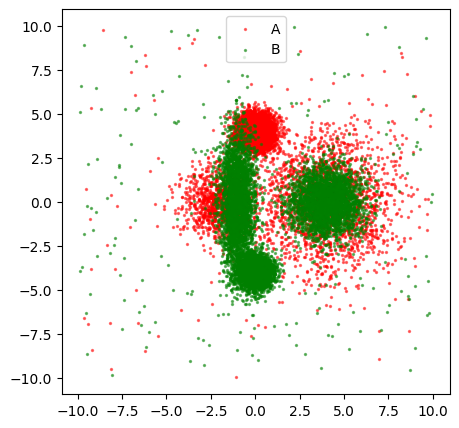
\includegraphics[width=\linewidth]{Figures/fused_data_2D_fcm.png}
		\caption[Application of fcm distance - fused data]{The two sets of images are shown in the figure. \vspace{3.50em}}
		\label{fig:fused_data_2D_fcm}
	\end{subfigure}
	\hfill
	\begin{subfigure}{0.45\linewidth}
		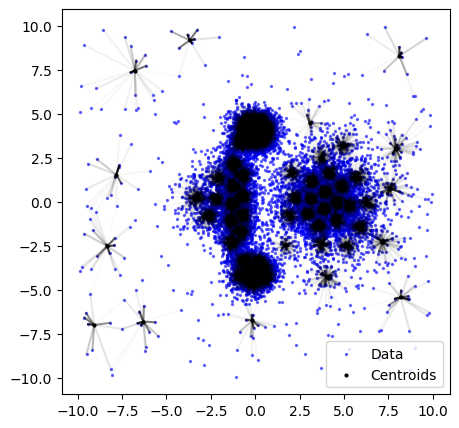
\includegraphics[width=\linewidth]{Figures/fcm_2D_fcm.png}
		\caption[Application of fcm distance - fcm application]{A clustering \gls{fcm} with $64$ centroids is shown in the figure; significant relationships between data and clusters are represented by means of segments.}
		\label{fig:fcm_2D_fcm}
	\end{subfigure}
	\begin{subfigure}{\linewidth}
		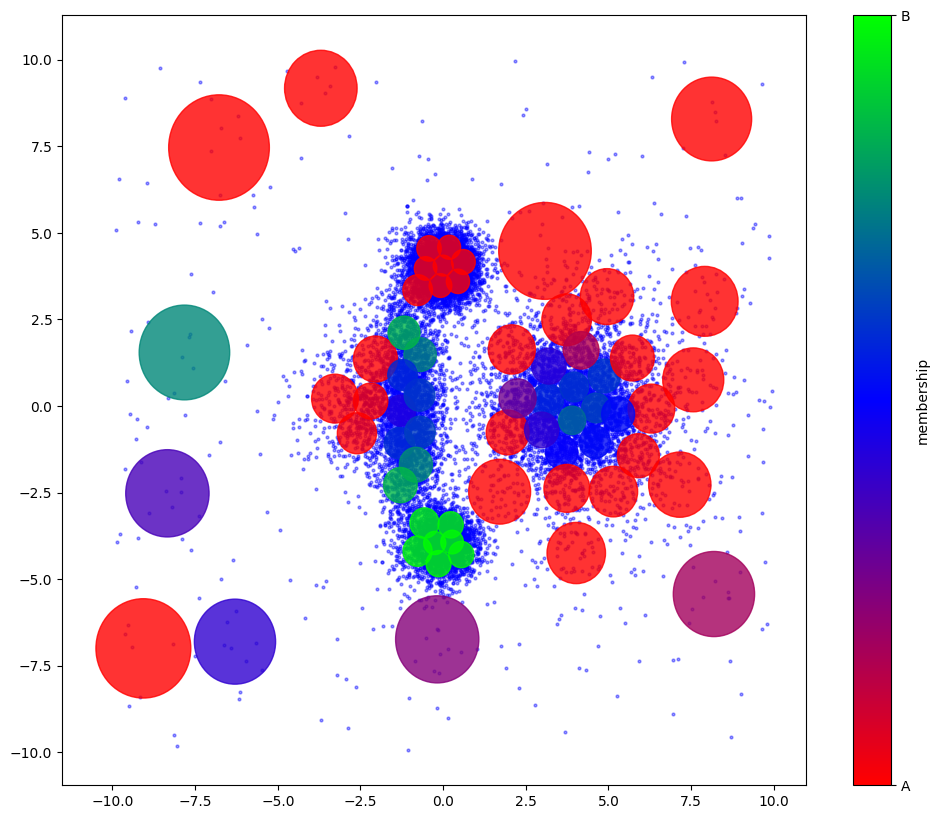
\includegraphics[width=\linewidth]{Figures/measure_2D_fcm.png}
		\caption[Application of fcm distance - discretisation]{Clusters are shown in the figure with an area covering the size of the cluster and a colour indicating its characterisation; in particular, the colour scale is mapped onto $\frac{\omega_A-\omega_B}{\omega_A+\omega_B}$.}
		\label{fig:measure_data_2D_fcm}
	\end{subfigure}
\end{figure}

\newpage
\noindent We calculate the Jaccard index:
\begin{itemize}
	\item $ |D_A| = 53.17 $ e $ |D_B| = 52.26 $
	\item $ |D_A\cap D_B| = 43.91 $ e $ |D_A \cup D_B| = 61.53 $
	\item $ J_{D_A,D_B} = 0.71 $
\end{itemize}
We estimate the integral and consequently the distance between the distributions:
\begin{itemize}
	\item $ \frac{\sum_c \left(\frac{r(c)-1}{r(c)+1}\right)^2 \mu(c)}{\sum_c \mu(c)} = 0.31 $
	\item $ (1 + J_{D_A, D_B})^{-1} = 0.58 $
	\item $ d(A,B) = 0.18 $
\end{itemize}
We observe that the result in the presence of noise is not very dissimilar to the result obtained with \gls{kmeans} in the absence of noise (see \cref{tab:kmeans_tessellation_comparison}). Another example is with $256$ nodes where the distance will be $0.38$ so again there are no noise-related problems.

\noindent We verify the potential of \gls{fcm} by examining the distances computed by \gls{kmeans} in the presence of noise:
\begin{itemize}
	\item $64$ nodes: the estimated distance is $0.12$ versus the previous $0.30$ from \gls{kmeans}.
	\item $256$ nodes: the estimated distance is $0.23$ versus the previous $0.34$  from \gls{kmeans}.
\end{itemize}
The reduction in distance is an expected phenomenon, as the noise is identical for both samples, thus making them more similar. \gls{fcm} can slightly clean the sets from noise and thus have a more accurate estimate.

\paragraph{\gls{gpu}}
%L'algoritmo presentato è una soluzione sequenziale per l'estrazione delle tessere. Esso lavora iterando attraverso le righe e le colonne dell'immagine, estrae le tessere di dimensioni $N \times N$ e le inserisce in una lista. Tuttavia, questo approccio ha un costo computazionale pari a $O(hwN^2)$.\\
\noindent The \cref{alg:MembershipUpdateSafe} shown is a sequential solution for \gls{fcm}. It works by iterating through the data and centroids to compute the membership matrix. However, this approach has a computational cost of $O(NCk)$.

%Per migliorare l'efficienza computazionale, si può ricorrere all'utilizzo del boost della GPU (General Purpose Graphics Processing Unit). Questo genere di operazioni è noto come GPGPU (General-Purpose computing on Graphics Processing Units). Sfruttare la potenza di calcolo parallelo offerta dalle GPU può notevolmente accelerare il processo di estrazione delle tessere.
\noindent To improve computational efficiency, the use of \gls{gpu} \gls{boost}ing can be employed. This kind of operation is known as \gls{gpgpu}. Exploiting the parallel computing power offered by a \gls{gpu} can greatly accelerate the process of comparison.

%La \gls{gpu}, o unità di elaborazione grafica, è un componente elettronico presente in ogni computer, in grado di eseguire un grande numero di operazioni in parallelo. Originariamente concepita per gestire l'interfaccia grafica nei videogiochi, la \gls{gpu} si trova tipicamente nelle schede grafiche, dove è in grado di visualizzare miliardi di pixel sullo schermo di ogni computer a velocità che la \gls{cpu} non può raggiungere.\\
\noindent The \gls{gpu} is an electronic component present in every computer, able to perform a large number of operations in parallel. Originally designed to handle the graphical interface in video games, the \gls{gpu} is capable of handling billions of pixels on any computer screen at speeds that the \gls{cpu} cannot achieve.

%Questo processore è costituito da migliaia di thread, organizzati gerarchicamente a livello hardware per massimizzarne le prestazioni:
%\begin{enumerate}[label=\roman*.]
%\item \gls{sm}: Esegue un kernel e consiste di numerosi warp;
%\item \gls{warp}: Esegue il kernel del suo stream e possiede una memoria condivisa tra i suoi thread, di solito $32$;
%\item \gls{thread}: Esegue il kernel del suo warp sincronizzandosi con gli altri \gls{thread} dello stesso \gls{warp} e possiede una propria memoria riservata nei suoi registri.
%\end{enumerate}
\noindent This processor is made up of thousands of threads, organised hierarchically at the hardware level to maximise performance:
\begin{enumerate}[label=\roman*.]
\item \gls{sm}: Runs a kernel and consists of numerous \gls{warp}s;
\item \gls{warp}: Runs the kernel of its stream and has shared memory between its threads, usually $32$;
\item \gls{thread}: Executes the kernel of its warp by synchronising with the other \gls{thread}s of the same \gls{warp} and has its own reserved memory in its registers.
\end{enumerate}
%La memoria alla quale può accedere una \gls{gpu} è suddivisa in diverse categorie, tra cui la memoria \textit{global}, \textit{shared}, \textit{cache} e \textit{register}. L'accesso a queste memorie da parte dei \gls{thread} del processore dipende dalla gerarchia dei \gls{thread} stessi. Ad esempio, la memoria \textit{global} è accessibile da ogni \gls{thread}, mentre la memoria \textit{shared} è accessibile solo dai \gls{thread} appartenenti allo stesso \gls{warp}.\\
\noindent The memory that a \gls{gpu} can access is divided into different categories, namely \textit{global}, \textit{shared}, \textit{cache} and \textit{register} memory. Access to these memories by the processor's \gls{thread}s depends on the hierarchy of the \gls{thread}s themselves. For example, the \textit{global} memory is accessible by every \gls{thread}, while the \textit{shared} memory is only accessible by \gls{thread}s in the same \gls{warp}.

%In un computer di alta fascia, è comune trovare schede video dotate di $14$ \gls{sm}, ognuno dei quali contiene $1024$ \gls{thread} suddivisi in $32$ \gls{warp}. Questo totale di $14336$ \gls{thread} può eseguire in parallelo lo stesso identico codice, consentendo un'elaborazione estremamente veloce delle immagini e di altre operazioni che richiedono un alto grado di parallelismo.\\
\noindent In a high-end computer, it is common to find a \gls{gpu} equipped with $14$ \gls{sm}, each of which contains $1024$ \gls{thread}s divided into $32$ \gls{warp}s. This total of $14336$ \gls{thread}s can execute the exact same code in parallel, permitting extremely fast processing of images and other operations requiring a high degree of parallelism.

%A partire dagli anni $2000$, l'uso delle \gls{gpu} si è esteso al campo del calcolo scientifico, introducendo importati concetti come la scalabilità e l'\gls{hpc}. Dal $2020$, sono disponibili sul mercato \gls{gpu} dedicate alle operazioni di intelligenza artificiale.\\
\noindent Since the $2000$s, the use of \gls{gpu} has extended to the field of scientific computing, introducing important concepts such as scalability and \gls{hpc}. Since $2020$, dedicated \gls{gpu} are available on the market for artificial intelligence operations.

%In \gls{Python}, esistono framework utili per l'utilizzo delle \gls{gpu}, come \textit{torch} e \textit{TensorFlow}, ampiamente impiegati nell'ambito della computer vision. Tuttavia, anche linguaggi come il \verb"C++" offrono dialetti che consentono di sfruttare queste potenti unità di calcolo. In questo contesto, si userà il dialetto CUDA.\\
\noindent In \gls{Python}, there are useful frameworks for the utilisation of \gls{gpu}, such as \textit{torch} and \textit{TensorFlow}, which are widely employed in the field of computer vision. However, also languages such as \verb "C++" offer dialects that allow these powerful computing units to be exploited. In this paper, the \gls{cuda} dialect will be used.
\footnote{for more details about GPU architecture, see\newline\url{https://researchcomputing.princeton.edu/support/knowledge-base/gpu-computing}}
\footnote{for more details about \gls{cuda} language, see\newline\url{https://docs.nvidia.com/cuda/}}

\bigskip
The integration of \gls{gpgpu} techniques would allow the workload to be distributed over several cores of the \gls{gpu}, thus reducing the time needed for clustering operations. This method is particularly advantageous when handling large amounts of data, as the \gls{gpu} can perform many operations in parallel, speed up computation to be $2000$ times faster than the \gls{cpu} could have done.

\noindent The sum of $N$ numbers can be performed in with computational cost $O(log(N))$. This is because in parallel the \gls{gpu} threads sum one half of the vector over another at the same instant and then repeat until they get a single component that will have only one number. This operation is called \textit{reduction} and we can see it in the \cref{alg:gpu_reduction}. This is just one detail of how the \gls{gpu} can reduce the asymptotic computational cost of an algorithm. Suffice it to say that thanks to reductions and strong parallelism, it is possible to multiply two $N\times K$ and $K\times M$ matrices with cost $O(log(K))$ instead of $O(NMK)$. In clustering many operations can be parallelised and \gls{fcm} in particular requires many sums and linear operations.

\noindent The limitations of \gls{gpu} are not only related to the execution of the same operations on all threads, but also to the nature of these operations. Normally, an instruction takes much longer to be executed by a \gls{gpu} than by a \gls{cpu}. Arithmetic instructions are the most efficient, while the use of conditions tends to be avoided.

\begin{algorithm}
\caption[Parallel algorithm for sum reduction]{Parallel algorithm for sum reduction.\\
	\begin{minipage}[t]{\linewidth}
		\textsc{INPUT}
		\begin{itemize}[noitemsep, topsep=0pt]
			\item[$\textnormal{v}$:] array of values
			\item[$\textnormal{N}$:] number of components
		\end{itemize}
		This algorithm sum all values of an array and write in $\textnormal{v}[0]$ the result. The array is not preserved, in this way the algorithm does not allocate new memory. The computational cost is $O(\log(N))$. In \cref{fig:gpu_reduction} an example over a vector with $7$ components.
	\end{minipage}
}
\begin{algorithmic}[1]
\Procedure{Kernel $\textnormal{i}$, SumReduction}{$\textnormal{v}$,$\textnormal{N}$}
    \State Let $S$ a shared vector with $2^k \geq N$ component
    \State $S[\textnormal{i}] \gets \textnormal{v}[\textnormal{i}]$ if $\textnormal{i}<\textnormal{N}$ else $0$
    \For{$L \gets 2^{k}/2,2^{k}/4,\dots,1$}
        \If{$\textnormal{i} < L$}
            \State $S[\textnormal{i}] \gets S[\textnormal{i}] + S[\textnormal{i}+L]$
        \EndIf
        \State require synchronisation between threads
    \EndFor
\EndProcedure
\label{alg:gpu_reduction}
\end{algorithmic}
\end{algorithm}

\begin{figure}[h]
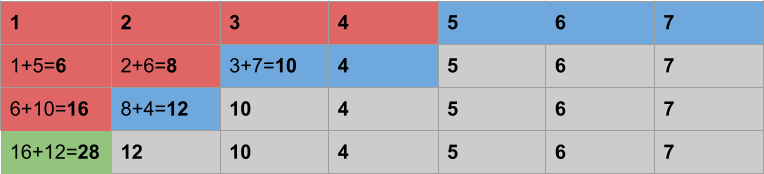
\includegraphics[width=\linewidth]{Figures/example_gpu_reduction.png}
\caption[Application of sum reduction]{We want to calculate the sum of the values in the first row. The idea is to divide the vector into $2$ regions, sum the components, and repeat over the new vector with half the size of the previous vector.}
\label{fig:gpu_reduction}
\end{figure}
